\subsection{The theory of PID}

\subsubsection{Principles of PID Control}

PID (Proportional-Integral-Derivative) control is a popular feedback control algorithm that is utilized in a variety of control systems. PID control is made up of three parts: proportional, integral, and derivative. The proportional term controls the process based on the current difference between the desired setpoint and the measured process variable. To decrease steady-state mistakes and improve system stability, the integral term accumulates past errors over time. The derivative term computes the error's rate of change and aids in dampening quick changes, improving response time and lowering overshoot. \cite{PIDbook}
\subsubsection{PID Control Loop}

The PID control loop is made up of four basic components: the process or plant under control, in this case roll and pitch, the process or plant under control, and the process or plant under control. A sensor or measurement device. The PID controller and the actuator. The IMU measures the process variable (angle) and compares it to the desired setpoint. The PID controller calculates the control signal based on the mistake, and the actuator alters the system accordingly. In this closed-loop feedback system, the control signal is continuously changed to keep the process variable close to the setpoint. \cite{PIDbook}
\subsubsection{Benefits of PID Control}

PID is a versatile and frequently used control algorithm that provides excellent control in a variety of applications. Other solutions exist, such as model predictive control, but they are less widespread and thus have a smaller community. \cite{Efheij2019}

\paragraph{Stability}PID control helps maintain system stability by continuously adjusting the control signal based on the error feedback. The proportional, integral, and derivative terms work together to provide a balance between stability and responsiveness. \cite{PIDbook}
\paragraph{Robustness}PID control is robust and effective in handling disturbances, noise, and external factors that may affect the system's performance. The integral term, in particular, helps eliminate steady-state errors caused by external disturbances. \cite{PIDbook}
\paragraph{Adaptability}PID control can be tuned and adjusted to optimize performance based on specific system requirements. The controller gains can be modified to enhance stability, reduce overshoot, or improve response time. \cite{PIDbook}
\paragraph{Simplicity}PID control is relatively easy to implement and understand. It offers a straightforward approach to control systems without requiring complex mathematical models or extensive computational resources. \cite{PIDbook}

\subsubsection{Ziegler-Nichols method}
The performance of a PID controller depends on appropriate tuning to match the characteristics of the controlled system. Tuning involves adjusting the proportional, integral, and derivative gains to achieve the desired response. 
To tune the quadrotor's PID Ziegler-Nichols method was used, as it is compromise between complexity and time. \cite{ZNPID}

The value of the proportional-only gain that allows the control loop to oscillate forever at steady state is used to calculate the ultimate gain, $K_u$ . This means that the gains from the I and D controllers are set to zero in order to determine the influence of P. It evaluates the robustness of the $K_c$ value in order to optimize it for the controller. The final period is another key number related with this proportional-only control tuning approach ($P_u$). The ultimate period is the amount of time it takes to complete one entire oscillation while the system is in steady state. These two parameters, $K_u$ and $P_u$, are employed to determine the controller's loop-tuning constants (P, PI, or PID). \cite{LibrePID}

\begin{figure}[H]
    \begin{center}
    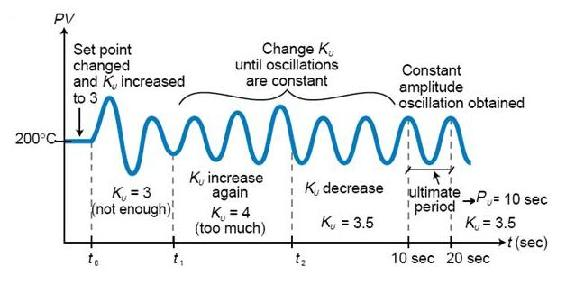
\includegraphics[scale=0.7]{pictures/control/pidexample}
    \end{center}
    \caption{Example of a system tuned using the Ziegler-Nichols method\cite{LibrePID}}
    \label{fig:znmethod}
\end{figure}

Ziegler-Nichols method steps are as follows:
\begin{enumerate}
    \item 
    Take out the integral and derivative actions. Set the integral time ($T_i$) to 999 or the highest number possible, and the derivative controller ($T_d$) to zero.
    \item 
    Change the set point to cause a slight perturbation in the loop. Increase or decrease the gain of the proportional until the oscillations have a constant amplitude.
    \item 
    Mark down the gain value ($K_u$) and period of oscillation ($P_u$).
    \item 
    Input these values into the Ziegler-Nichols equations to find the controller settings. (See Table \ref*{table.pidconstants})
\end{enumerate}

\begin{table}[H]
    \begin{tabular}{llllll}
    \textbf{Control Type}   & $K_p$        & $T_i$     & $T_d$      & $K_i$           & $K_d$\\
    \textbf{P}              & 0.5$K_u$     & –         & –          & –               & –\\
    \textbf{PI}             & 0.45$K_u$    & 0.83$T_u$ & –          & 0.54$K_u$/$T_u$ & – \\
    \textbf{PD}             & 0.8$K_u$     & –         & 0.125$T_u$ & –               & 0.1$K_u$$T_u$ \\
    \textbf{classic PID}    & 0.6$K_u$     & 0.5$T_u$  & 0.125$T_u$ & 1.2$K_u$/$T_u$  & 0.075$K_u$$T_u$ \\
    \textbf{some overshoot} & 0.33$K_u$    & 0.5$T_u$  & 0.33$T_u$  & 0.66$K_u$/$T_u$ & 0.11$K_u$$T_u$ \\
    \textbf{no overshoot}   & 0.2$K_u$     & 0.5$T_u$  & 0.33$T_u$  & 0.4$K_u$/$T_u$  & 0.066$K_u$$T_u$ \\
    \end{tabular}
\caption{Formulas for determening the PID constants via Ziegler-Nichols}
\label{table.pidconstants}
\end{table}
